\subsection{Turtlebot Mecanum}
\label{partie:turtlebot}

\begin{wrapfigure}{r}{0.25\textwidth}
    \vspace{-0.2cm} 
    \centering
    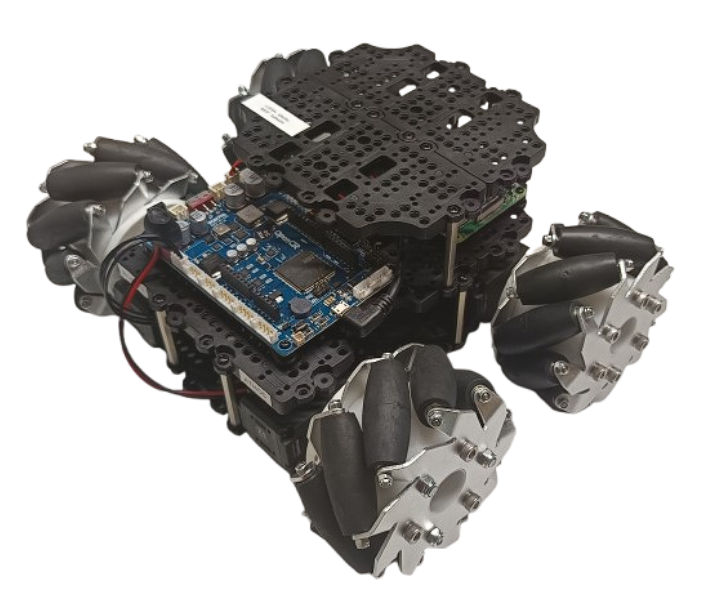
\includegraphics[width=\linewidth]{10-Descriptions_réalisations/Outils/pic/Mecanum.png}
    \caption{TurtleBot Mecanum}
    \label{fig:mecanum}
    \vspace{-0.5cm} 
\end{wrapfigure}

Comme mentionné précédemment, avant d'implémenter le programme de contrôle événementiel sur des drones, celui-ci sera dans un premier temps développé et testé sur des robots mobiles de type Turtlebot, équipés de roues Mecanum (Figure \ref{fig:mecanum}).
Les roues Mecanum sont des roues particulières, composées de plusieurs galets montés en biais autour de leur circonférence, ce qui permet au robot de réaliser des mouvements dans toutes les directions du plan en combinant les vitesses de rotation de chaque roue. Ce type de robot est dit \textit{holonome}.
\noindent La cinématique des robots Mecanum est donnée dans \cite{tan_research_2021}.

Chaque robot est composé de quatre moteurs Dynamixel, d'une carte OpenCR assurant le pilotage bas niveau, et d'une Raspberry Pi 4 servant d'unité de calcul principale.
Ils ont été conçus et programmés initialement sous \gls{ros1} dans le cadre d'un projet de 5ème année à l'INSA Strasbourg. Trois robots étaient disponibles au début du stage, portant les noms des trois mousquetaires : Athos, Porthos et Aramis \cite{vrignaud_swarm_2025}. Trois robots supplémentaires ont été construits et programmés durant le stage : Dartagnan, Edmon et Mercedes.

% Nécessite \usepackage{tikz}
\begin{figure}[h]
    \centering
    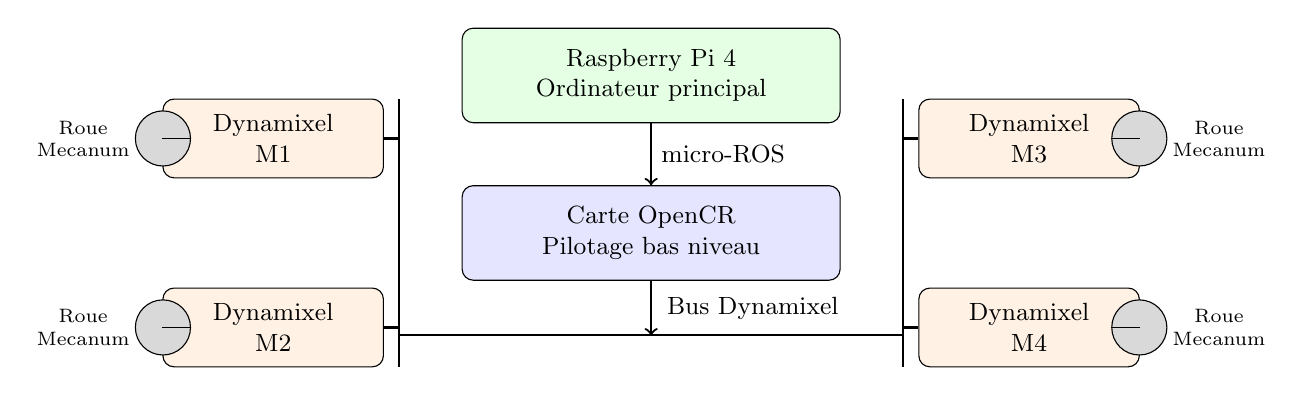
\begin{tikzpicture}[font=\small]
        % Blocs principaux
        \node[draw, rounded corners, fill=green!10, minimum width=4.8cm, minimum height=1.2cm, align=center] (rpi) at (0,0) {Raspberry Pi 4\\Ordinateur principal};
        \node[draw, rounded corners, fill=blue!10, minimum width=4.8cm, minimum height=1.2cm, align=center] (opencr) at (0,-2) {Carte OpenCR\\Pilotage bas niveau};

        % Lien RPi -> OpenCR
        \draw[->, thick] (rpi) -- node[right]{micro-ROS} (opencr);

        % Bus Dynamixel (gauche et droite)
        \coordinate (busLt) at (-3.2,-0.3);
        \coordinate (busLb) at (-3.2,-3.7);
        \coordinate (busRt) at ( 3.2,-0.3);
        \coordinate (busRb) at ( 3.2,-3.7);
        \draw[thick] (busLt) -- (busLb);
        \draw[thick] (busRt) -- (busRb);
        % Bus série: relie les deux montants, plus bas
        \def\ybus{-3.3}
        \draw[thick] (-3.2,\ybus) -- ( 3.2,\ybus);

        % Connexions OpenCR -> bus
        \draw[->, thick] (opencr.south) -- node[pos=0.5, right, xshift=2pt]{Bus Dynamixel} (0,\ybus);
        % \draw[->, thick] (opencr.east) -- ( 3.2,-2); % retiré: bus série, une seule connexion

        % Positions des moteurs (deux à gauche, deux à droite)
        \def\yt{-0.8}
        \def\yb{-3.2}

        \node[draw, rounded corners, fill=orange!10, minimum width=2.8cm, minimum height=1.0cm, align=center] (mL1) at (-4.8,\yt) {Dynamixel \\M1};
        \node[draw, rounded corners, fill=orange!10, minimum width=2.8cm, minimum height=1.0cm, align=center] (mL2) at (-4.8,\yb) {Dynamixel \\M2};
        \node[draw, rounded corners, fill=orange!10, minimum width=2.8cm, minimum height=1.0cm, align=center] (mR1) at ( 4.8,\yt) {Dynamixel \\M3};
        \node[draw, rounded corners, fill=orange!10, minimum width=2.8cm, minimum height=1.0cm, align=center] (mR2) at ( 4.8,\yb) {Dynamixel \\M4};

        % Connexions bus -> moteurs
        \draw[thick] (-3.2,\yt) -- (mL1.east);
        \draw[thick] (-3.2,\yb) -- (mL2.east);
        \draw[thick] ( 3.2,\yt) -- (mR1.west);
        \draw[thick] ( 3.2,\yb) -- (mR2.west);

        % Roues Mecanum (à l'extérieur, formant un "carré" autour du coeur RPi/OpenCR)
        \node[draw, circle, fill=gray!30, minimum size=0.7cm] (wL1) at (-6.2,\yt) {};
        \node[draw, circle, fill=gray!30, minimum size=0.7cm] (wL2) at (-6.2,\yb) {};
        \node[draw, circle, fill=gray!30, minimum size=0.7cm] (wR1) at ( 6.2,\yt) {};
        \node[draw, circle, fill=gray!30, minimum size=0.7cm] (wR2) at ( 6.2,\yb) {};
        \draw (mL1.west) -- (wL1.east);
        \draw (mL2.west) -- (wL2.east);
        \draw (mR1.east) -- (wR1.west);
        \draw (mR2.east) -- (wR2.west);

        % Légendes roues (discrètes)
        \node[anchor=east, font=\scriptsize, align=center] at (-6.5,\yt) {Roue \\ Mecanum};
        \node[anchor=east, font=\scriptsize, align=center] at (-6.5,\yb) {Roue \\ Mecanum};
        \node[anchor=west, font=\scriptsize, align=center] at ( 6.5,\yt) {Roue \\ Mecanum};
        \node[anchor=west, font=\scriptsize, align=center] at ( 6.5,\yb) {Roue \\ Mecanum};
    \end{tikzpicture}
    \caption{Schéma fonctionnel du TurtleBot Mecanum}
    \label{fig:tb-mecanum-schema}
\end{figure}


Les six robots ont été re-programmés en \gls{ros2} . Cela nécéssitait le passage vers le système d'exploitation Ubuntu 22.04 (contre 20.04 pour la version ROS1), ainsi qu'une reprogrammation quasi-totale de la carte OpenCR, qui utilise désormais la librairie Micro-ROS pour communiquer avec la Raspberry Pi. La carte OpenCR est programmée en C++, tandis que les noeuds \gls{ros2} tournent sur la Raspberry Pi via des programmes Python pour le pilotage haut niveau du robot. Aussi, un \textit{service} Linux a été créé pour lancer automatiquement la communication Micro-ROS au démarrage du robot. Les moteurs Dynamixels sont pilotés via un bus série, et chacun doit avoir une adresse unique sur le bus (Figure \ref{fig:tb-mecanum-schema}). Pour cela, un logiciel nommé Dynamixel Wizard est utilisé.
Le tutoriel de migration vers \gls{ros2} est disponible en annexe (annexe \ref{chap:mecanum}). 


\noindent \underline{Note :} Les Raspberry Pi des robots Athos, Porthos et Aramis ont une plus grande capacité de stockage que Dartagnan, Edmon et Mercedes, et sont programmés avec la version Desktop d'Ubuntu 22.04, tandis que les trois autres sont programmés avec la version Server. Cela n'a pas d'impact sur le fonctionnement direct des robots, mais cela implique des différences de consommation de ressources, notamment en mémoire vive (\gls*{ram}), car la version Server est beaucoup plus légère que la version Desktop.
Un tableau récapitulatif des configurations des robots est donné ci-dessous (\ref{tab:config-robots}).
\begin{table}[h]
    \centering
    \small
    \begin{tabular}{|l|l|l|l|l|}
        \hline
        Robot & Ubuntu & \gls*{ram} (\gls*{go}) & \gls*{cpu} & Stockage (\gls*{go}) \\
        \hline
        Aramis &  22.04 Desktop & 4 & 64-bit quad-core & 32 \\
        Athos &  22.04 Desktop & 4 & 64-bit quad-core & 32 \\
        Porthos &  22.04 Desktop & 4 & 64-bit quad-core & 32 \\
        d'Artagnan &  22.04 Server & 2 & 64-bit quad-core & 16 \\
        Edmon &  22.04 Server & 2 & 64-bit quad-core & 16 \\
        Mercedes &  22.04 Server & 2 & 64-bit quad-core & 16 \\
        \hline
    \end{tabular}
    \caption{Configurations matérielles et logicielles des robots}
    \label{tab:config-robots}
\end{table}



